\section{Conclusion and Discussion}

\subsection{Natural angular frequency}

Although by theory amplitude doesn't affect the period, as the amplitude gets
larger, the negative work done by the frictional force isn't negligible.  
Thus, we need to keep the amplitude the same for every test to reduce this
influence factor.

The third measurement of ten periods is obviously smaller than the other three,
which might result from a severely different amplitude.

On the other hand, by measuring 10 times of T, the experimental value of
$\omega_0$ is quite precise (with small deviation).
Still, $u_{10T,r}=0.07\%$, that means our experiment setup works pretty well.

For recommendation, I think introducing a control system for the amplitude in
addition to bare hand can bring more precision.



\subsection{Damping coefficient}

The damping coefficient is calculated from dividing the decreasing
amplitude and log it.
When calculating the damping coefficient, successive difference method is applied
to reduce the deviation. 

For more precision than successive difference method, we could use curve fitting,
thus the whole list can be used to determine the damping coefficient $\beta$
from $\theta_n=\theta_0e^{-\beta (nT)}$, instead of only using 5 groups of
isolated points. 

\begin{figure}[H]
\centering
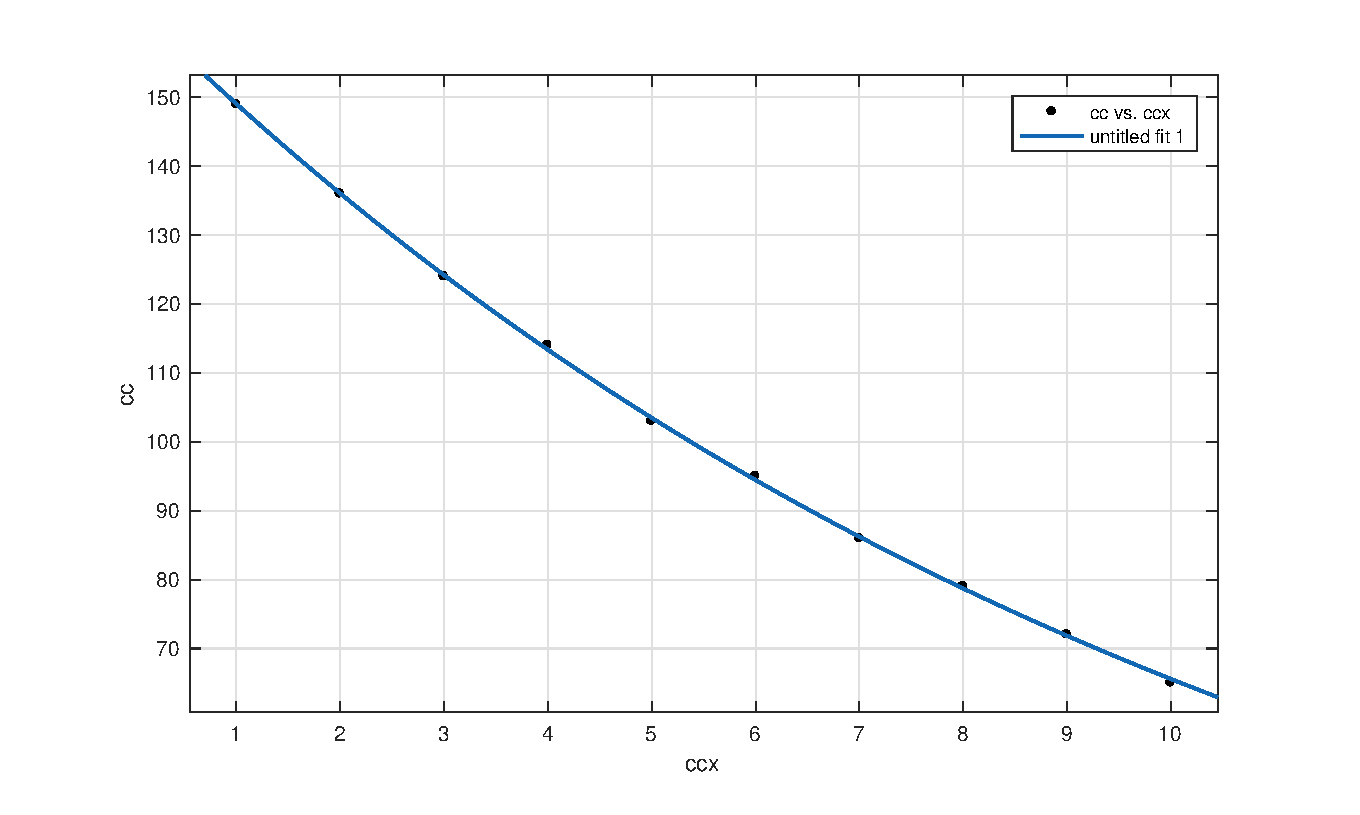
\includegraphics[width=0.7\textwidth]{matlab/p3}
\caption{Curve fitting example}
\end{figure}

And we can find the b of the curve, which is $-0.09125$
Comparing $- 5\times b =  0.4562 $ with $\beta = 0.4558$
$$ u_{\beta,r}=  0.0878 \% $$

We can reach a conclusion that although curve fitting can introduce more precise
process, the present method is quite accurate.


% NOTE:DONE

\subsection{$\varphi$ vs. $\omega$}

Both of the $\varphi$ vs. $\omega$ curve are in the shape of arc
cotangent (see Figure~\ref{phi}).
In theory we know that for the smaller damping coefficient, the left side curve
of $\omega/\omega_0=1.0$ is higher than the other and the right side curve is
lower than that. 

My fit curve quit matches what a arc cotangent line looks like, one curve higher
before the intersection point and lower after the intersection point.
The time duration will be longer to reach the stable situation. 
The second half of phase points number lesser than the first one because it's
hard to predict how the $\varphi$ goes. 

For recommendation, it hurts for us to bear the flashlight for reading the phase
data. 
Electronic devices such as a camera can be introduced to record the data,
instead of directly reading the data with human eyes.

\subsection{$\theta_{st}$ vs. $\omega$}

The shape of both curve meets our expectation (in Figure~\ref{theta}).

In the figure, the curve's shape and position meet the expectation, that is
damping 3's damping coefficient is greater than damping 2's.
And the curve is same as the theory.

From the figure, it's obvious whether the peaks occur on the left or right hand
side of the straight line $\omega/\omega_0=1.0$ for Damping Selection 2, but
hard for Damping Selection 3.
It is because that the deviation is smaller for Damping Selection 3.
In theory, the peaks should occur on the slightly left of the straight
line. 
